Most Chip Multiprocessors (CMPs) share parts of the memory system to improve resource utilization.
In particular, the last level cache (LLC) is commonly shared between processor cores.
This design choice makes destructive cache interference possible which reduces performance and may cause problems such as missed deadlines, priority inversion, unpredictable interactive performance and non-compliance with service level agreements \cite{dubois13}.
For this reason, computer architecture researchers have proposed a large number of microarchitectural techniques that partition the LLC between competing processes (e.g.\ \cite{suh02,dynPartofSharedCacheMemory,utilityBasedCachePartitioning,haakonHiPC,jaleel08,xie09,jaleel10,xie10,manikantan11,sanchez11,sundararajan12,manikantan12,duong12,hasenplaugh12,albericio13}).
Given the large amount of cache partitioning research, it is common to reuse previously proposed ideas in new schemes.
Unfortunately, it can be hard to identify this reuse without understanding the work in detail.
In this work, we propose a classification scheme that can identify such overlap and thus help future architects avoid reinventing the wheel.

We loosely define the cache partitioning problem as the task of managing shared LLC capacity in a process-aware manner with the aim of achieving a performance-related goal.
We differentiate between \textit{explicit} and \textit{implicit} cache partitioning.
In explicit cache partitioning, each running process is assigned an LLC quota which determines the minimum amount of cache space available to each process (e.g.\ \cite{suh02,dynPartofSharedCacheMemory,utilityBasedCachePartitioning,haakonHiPC,xie09}).
With implicit partitioning, LLC space is managed by process-aware replacement, insertion or promotion policies without assigning a specific quota to each process (e.g.\ \cite{jaleel08,jaleel10,manikantan11,albericio13}).

The first contribution of this work is a method for classifying cache partitioning techniques.
All cache partitioning techniques contain a \textit{policy} which defines the goal to be achieved with partitioning and \textit{mechanisms} that are the primitives used to implement the policy \cite{virtualPrivateMachines}.
The three most common policies are to minimize the total number of LLC misses, to provide \textit{Quality of Service (QoS)} by ensuring that the performance of one or more processes is kept above a certain level or to provide \textit{fairness} by distributing the performance loss due to interference equally among the running threads.
Cache partitioning techniques also commonly use a \textit{feedback} mechanism and a \textit{partitioning} mechanism.
The feedback mechanism gathers information regarding the cache requirements of the currently running processes while the partitioning mechanism is used to select and enforce partitions (explicitly or implicitly).
Examples of feedback mechanisms are \textit{Auxilliary Tag Directories (ATDs)} \cite{utilityBasedCachePartitioning,haakonHiPC}, set dueling \cite{jaleel10} and marginal gain counters \cite{dynPartofSharedCacheMemory,suh02}.
Partitioning mechanism examples are way partitioning  \cite{utilityBasedCachePartitioning}, modified promotion and insertion policies (e.g.\ \cite{xie09}) and modified replacement policies (e.g.\ \cite{jaleel10, albericio13}).

We apply our classification scheme to previously proposed dynamic miss minimizing partitioning techniques.
This is to the best of our knowledge the first attempt at systematically classifying cache partitioning techniques.
The main observation resulting from this classification is that it is common to apply previously proposed ideas in some form.
For instance, the ATD feedback mechanism has been used extensively \cite{utilityBasedCachePartitioning,haakonHiPC,xie09,xie10,sanchez11,sundararajan12,manikantan12}.
This is not surprising given the large number of proposed techniques targeting cache partitioning, but for science to progress it is critical that these overlaps are clearly identified.
Thus, our classification scheme enable architects to clearly separate their novel ideas from previous work.

The second contribution of this work is a quantitative investigation of the performance of 5 high-impact cache partitioning techniques that collectively cover the current design space of miss minimizing partitioning techniques targeted at monolithic LLCs \magnus{verify that this is correct}.
Concretely, we implemented TADIP \cite{jaleel08}, DRRIP \cite{jaleel10}, UCP \cite{utilityBasedCachePartitioning}, PIPP \cite{xie09} and PriSM \cite{manikantan12}.
The baseline is a conventional LRU-managed shared LLC.
\magnus{What did we find?}
\magnus{Add the progression over time plot here?}
We aim to provide our implementations to the research community.

\magnus{Add outline of the work? Do we need it?}

\runar{Line plot, not shown PIPP 16 cores 0.54}

\begin{figure*}[t]
\centering
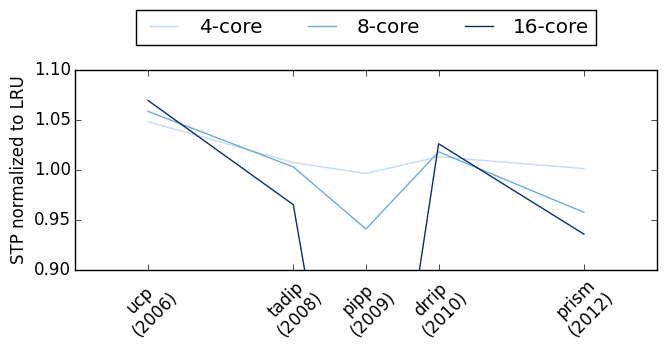
\includegraphics[width=\columnwidth]{figures/results/year-comp}
\caption{Average algorithm performance measured in STP normalized to LRU by year of publication. (Not shown 16-cores PIPP 0.54)}
\label{fig:yearlyComparison}
\end{figure*}

% Previous "meta analyses", can we get them in somewhere: \cite{microlib,comparingPrevalingSimulationTechniques,desmet10}).